\section{Aylana bo`ylab notekis harakat}


\begin{enumerate}

\item Moddiy nuqta aylana bo‘ylab tekis harakatlanmoqda. Uning tezlik va tezlanish vektorlari orasidagi burchak qanday?
\begin{enumerate}[label=\Alph*)]
\item $180^\circ$
\item $90^\circ$
\item $60^\circ$
\item $30^\circ$

\end{enumerate}

\item Avtomobil radiusi 50 m bo‘lgan aylanani $40^\circ$ ga mos yoyini 4 m/s, $60^\circ$ mos yoyini 6 m/s, $70^\circ$ mos yoyini 7 m/s va qolgan qismini 8 m/s tezlik bilan o‘tdi. Avtomobilning butun aylanadagi o‘rtacha tezligini toping (km/soat).
\begin{enumerate}[label=\Alph*)]
\item 2,15
\item 24,1
\item 36
\item 42,1

\end{enumerate}

\item Aylana bo‘ylab harakatlanayotgan jismning boshlang‘ich burchak tezligi 3 rad/s va burchak tezlanishi 0,1 rad/$s^2$. U 0,5 s da qancha aylana yoyi chizadi?
\begin{enumerate}[label=\Alph*)]
\item $86,7^\circ$
\item $80,7^\circ$
\item $60,7^\circ$
\item $90^\circ$

\end{enumerate}

\item Aylana bo‘ylab tekis tezlanuvchan harakat qilayotgan moddiy nuqtaning boshlang‘ich burchak tezligi 3 rad/s, burchak tezlanishi 0,1 rad/$s^2$. Uning 5 s dan keyingi burchak tezligini toping (rad/s).
\begin{enumerate}[label=\Alph*)]
\item 2,5
\item 4
\item 3,5
\item 2

\end{enumerate}

\item Aylana bo‘ylab tekis tezlanuvchan harakat qilayotgan moddiy nuqtaning boshlang‘ich burchak tezligi 4 rad/s, burchak tezlanishi 0,2 rad/$s^2$. Uning 4 s dan keyingi burilish burchagini toping (rad).
\begin{enumerate}[label=\Alph*)]
\item 17,6
\item 16
\item 1,6
\item 1,75

\end{enumerate}

\item Jism aylana bo‘ylab $\omega = 2 + 0,5t$ tenglama bilan ifodalanadigan burchak tezlik bilan harakat qilmoqda. U 20 s da necha marta aylanadi?
\begin{enumerate}[label=\Alph*)]
\item 62
\item 22
\item 42
\item 32

\end{enumerate}

\item Boshlang‘ich burchak tezligi 3 rad/s va burchak tezlanishi 0,5 rad/$s^2$ bo‘lgan jism aylana bo‘ylab tekis tezlanuvchan harakat qilmoqda. Aylana radiusi 5 dm bo‘lsa, 6 s dan keyingi chiziqli tezlikni toping (m/s).
\begin{enumerate}[label=\Alph*)]
\item 3
\item 2
\item 6
\item 8

\end{enumerate}

\item Tinch holatdan boshlab aylana bo‘ylab 0,4 rad/$s^2$ burchak tezlanish bilan harakatlanayotgan moddiy nuqtaning 20 s dan keyingi chiziqli tezligini toping (m/s). Aylananing radiusi 5 m.
\begin{enumerate}[label=\Alph*)]
\item 40
\item 20
\item 10
\item 5

\end{enumerate}

\item Egri chiziqli harakatda oniy tezlik vektorining yo‘nalishi qanday?
\begin{enumerate}[label=\Alph*)]
\item bunday harakatda oniy tezlik yo‘nalishini aniqlab bo‘lmaydi.
\item trayektoriyaga o‘tkazilgan urinma bo‘ylab.
\item egri chiziq radiusiga urinma bo‘ylab.
\item egri chiziq radiusi bo‘yicha markazdan.

\end{enumerate}

\item Jismning $AB$ trayektoriya bo‘ylab harakatlanishi natijasida uning tezligi $\vec{v}_1$ dan $\vec{v}_2$ gacha o‘zgaradi. Berilgan chizmada $B$ nuqtadagi $\vec{v}_2$ tezlik vektori $A$ nuqtaga o‘ziga parallel ko‘chirilgan. O‘rtacha tezlanish vektori qanday yo‘nalgan bo‘ladi?

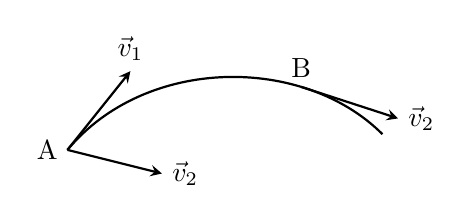
\begin{tikzpicture}[>=stealth, scale=2]
    % Trayektoriya (A dan B gacha bo'lgan egri chiziq)
    \draw[thick] (0,0) .. controls (0.5,0.6) and (1.5,0.6) .. (2,0.1);

    % Nuqtalar va ularning nomlari
    \node[left] at (0,0) {A};
    \node[above] at (1.485,0.4) {B};
    
    % v1 vektori - A nuqtada trayektoriyaga urinma holatda
    \draw[->, thick] (0,0) -- (0.4,0.5) node[above] {$\vec{v}_1$};

    % v2 vektori - B nuqtada trayektoriyaga urinma holatda
    % (B nuqtasi taxminan koordinatalari hisobga olindi)
    \draw[->, thick] (1.485,0.4) -- (2.1,0.2) node[right] {$\vec{v}_2$};

    % v2 vektorining A nuqtaga parallel ko'chirilgan holati
    % Yo'nalishi yuqoridagi v2 bilan bir xil
    \draw[->, thick] (0,0) -- (0.6,-0.15) node[right] {$\vec{v}_2$};

\end{tikzpicture}

\begin{enumerate}[label=\Alph*)]
\item $v_1$ vektor yo‘nalishiga mos yo‘nalgan.
\item $v_2$ vektor yo‘nalishiga mos yo‘nalgan.
\item $v_2$ vektor uchidan $v_1$ vektor uchiga qarab yo‘nalgan.
\item $v_1$ vektor uchidan $v_2$ vektor uchiga qarab yo‘nalgan.

\end{enumerate}

\item Jismning urinma tezlanishi 5 m/$s^2$ va natijaviy tezlanishi 10 m/$s^2$. Uning markazga intilma tezlanishini toping (m/$s^2$).
\begin{enumerate}[label=\Alph*)]
\item $5\sqrt{3}$
\item $5\sqrt{5}$
\item 5
\item 15

\end{enumerate}

\item Moddiy nuqta radiusi 3 m bo‘lgan aylana bo‘ylab 4 rad/s burchak tezlik bilan tekis harakatlanmoqda. Uning tangensial tezlanishini toping (m/$s^2$).
\begin{enumerate}[label=\Alph*)]
\item 48
\item 0
\item 24
\item 1,33
\end{enumerate}

\item Moddiy nuqta radiusi 20 sm bo‘lgan aylana bo‘ylab 5 sm/$s^2$ urinma tezlanish bilan tekis tezlanuvchan harakat qilmoqda. Harakat boshlangandan keyin qancha vaqt (s) o‘tgach normal (markazga intilma) tezlanishi, urinma tezlanishdan 2 marta katta bo‘ladi?
\begin{enumerate}[label=\Alph*)]
\item 2,78
\item 2,20
\item 1,07
\item 3,48

\end{enumerate}

\item Jism tangensial tezlanishi 6 m/$s^2$, markazga intilma tezlanishi 8 m/$s^2$ ga teng bo‘lsa, uning natijaviy tezlanishi necha m/$s^2$ ga teng?
\begin{enumerate}[label=\Alph*)]
\item 6
\item 8
\item 10
\item 2

\end{enumerate}

\item Gorizontal sirtda harakatlanayotgan moddiy nuqtaning tezligi va tezlanishi orasidagi burchak $\pi/3$ ga teng. Nuqtaning harakat xarakteri qanday?
\begin{enumerate}[label=\Alph*)]
\item to‘g‘ri chiziqli notekis
\item to‘g‘ri chiziqli tekis
\item egri chiziqli notekis
\item egri chiziqli tekis
\end{enumerate}

\item Moddiy nuqta radiusi 4 m bo‘lgan aylana bo‘ylab boshlang‘ich 2 rad/s burchak tezlik va 2 rad/$s^2$ burchak tezlanish bilan tekis tezlanuvchan harakatlanmoqda. Uning 5 s dan keyingi normal tezlanishni tangensial tezlanishga nisbatini toping.
\begin{enumerate}[label=\Alph*)]
\item 72
\item 48
\item 12
\item 24

\end{enumerate}

\item Diametri 100 sm bo‘lgan g‘ildirak gardishidagi $A$ nuqta 6 m/s tezlik bilan tekis aylanma harakat qilayotgan edi. Tormozlanish natijasida $A$ nuqta 2 m/$s^2$ tangensial tezlanish bilan harakat qila boshladi. Tormozlanish boshlanganidan 2,5 s o‘tgach $A$ nuqtaning tezlik vektori bilan tezlanish vektori orasidagi burchak necha gradusga teng bo‘ladi?
\begin{enumerate}[label=\Alph*)]
\item $90^\circ$
\item $45^\circ$
\item $135^\circ$
\item $120^\circ$
\end{enumerate}

\item Radiusi $\sqrt{3}$ m bo‘lgan g‘ildirak gardishidagi $A$ nuqta 4,2 m/s tezlik bilan tekis aylanma harakat qilayotgan edi. Tormozlanish natijasida $A$ nuqta 3 m/$s^2$ tangensial tezlanish bilan harakat qila boshladi. Tormozlanish boshlanganidan 0,4 s o‘tgach $A$ nuqtaning tezlik vektori bilan tezlanish vektori orasidagi burchak necha gradusga teng bo‘ladi?
\begin{enumerate}[label=\Alph*)]
\item $90^\circ$
\item $45^\circ$
\item $135^\circ$
\item $120^\circ$
\end{enumerate}

\item Rasmda ko‘rsatilgan g‘ildirak $A$ nuqtasining yerga nisbatan tezligi 3 m/s ga teng. $S$ nuqtaning yerga nisbatan tezligi -2 m/s ga teng. Aylana diametri 1 m ga teng va u yerda sirpanib dumalaydi. G‘ildirak gardishining markazga intilma tezlanishini toping (m/$s^2$).

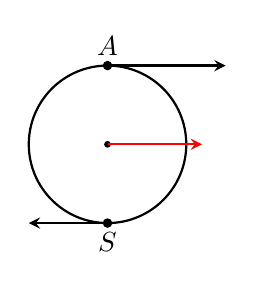
\begin{tikzpicture}[>=stealth, scale=1]
    % G'ildirak (aylana)
    \draw[thick] (0,0) circle (1);
    
    % Markaziy nuqta
    \filldraw (0,0) circle (1pt);
    
    % Nuqtalar: A (tepada) va S (pastda)
    \filldraw (0,1) circle (1.5pt) node[above] {$A$};
    \filldraw (0,-1) circle (1.5pt) node[below] {$S$};
    
    % Tezlik vektorlari (manbadagi rasmga va fizik qiymatlarga mos holda)
    
    % A nuqtadagi tezlik (3 m/s, o'ngga yo'nalgan) [1]
    \draw[->, thick] (0,1) -- (1.5,1);
    
    % Markazdagi tezlik (v_c = (3-2)/2 = 0.5 m/s, o'ngga yo'nalgan)
    \draw[->, thick,red] (0,0) -- (1.2,0);
    
    % S nuqtadagi tezlik (-2 m/s bo'lgani uchun chapga yo'nalgan) [1]
    \draw[->, thick] (0,-1) -- (-1,-1);

\end{tikzpicture}

\begin{enumerate}[label=\Alph*)]
\item 12,5
\item 50
\item 8
\item 18
\end{enumerate}

\item Diametri 100 sm bo‘lgan g‘ildirak gardishidagi $A$ nuqta 4,8 m/s tezlik bilan tekis aylanma harakat qilayotgan edi. Tormozlanish natijasida $A$ nuqta 3 m/$s^2$ tangensial tezlanish bilan harakat qila boshladi. Tormozlanish boshlanganidan 0,6 s o‘tgach $A$ nuqtaning tezlik vektori bilan tezlanish vektori orasidagi burchak necha gradusga teng bo‘ladi?
\begin{enumerate}[label=\Alph*)]
\item $90^\circ$
\item $90^\circ + \text{arcctg } 6$
\item $45^\circ$
\item $120^\circ$

\end{enumerate}

\end{enumerate}



\begin{table}[h!]
\centering
\caption{11. Aylana bo'ylab notekis harakat bo'limi uchun to'g'ri javoblar jadvali}
\begin{tabular}{|c|c|c|c|c|c|c|c|c|c|c|}
\hline
\textbf{Savol №} & 1 & 2 & 3 & 4 & 5 & 6 & 7 & 8 & 9 & 10 \\ \hline
\textbf{Javob}   & B & B & A & C & A & B & A & A & B & D \\ \hline
\hline
\textbf{Savol №} & 11 & 12 & 13 & 14 & 15 & 16 & 17 & 18 & 19 & 20 \\ \hline
\textbf{Javob}   & A & B & A & C & C & A & C & D & A & B \\ \hline
\end{tabular}
\end{table}








\section{Massa va zichlik}

\begin{enumerate}

\item Massasi $20$ kg bo‘lgan toshning hajmi $5$ l ga teng.
Uning zichligini toping $(\text{kg/m}^3)$.

\begin{enumerate}[label=\Alph*)]
\item 4000
\item 2000
\item 3000
\item 5000
\end{enumerate}


\item Uzunligi $30$ cm, eni $5$ cm va qalinligi $2$ cm bo‘lgan
jismning massasi $1.2$ kg ga teng.
Shu jismning zichligini toping $(\text{g/cm}^3)$.

\begin{enumerate}[label=\Alph*)]
\item 1
\item 2
\item 4
\item 0.8
\end{enumerate}


\item $18$ kg muzning hajmini va erigandan keyingi
hajmini toping $(l)$. $\rho_{\text{muz}} = 900\ \text{kg/m}^3, \quad \rho_{\text{suv}} = 1000\ \text{kg/m}^3$ 

\begin{enumerate}[label=\Alph*)]
\item 12; 18
\item 18; 18
\item 20; 20
\item 20; 18
\end{enumerate}


\item Parijdagi po‘latdan yasalgan, balandligi $300$ m
bo‘lgan Eyfel minorasining massasi $7200$ t.

Bu minoraning zichligi po‘latnikidan $2$ marta kichik
bo‘lgan moddadan yasalgan, balandligi $30$ cm
bo‘lgan modelining massasi qanday bo‘ladi?

\begin{enumerate}[label=\Alph*)]
\item 3.6 t
\item 3.6 kg
\item 360 g
\item 3.6 g

\end{enumerate}


\item Rasmda bir xil massali turli xil suyuqliklar
solingan uchta idish tasvirlangan.

Suv, spirt va simob qaysi idishlarda ekanligini aniqlang.

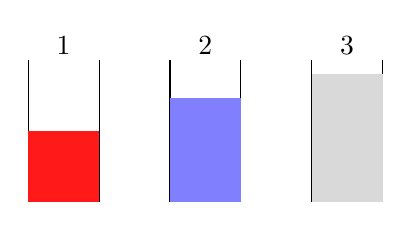
\begin{tikzpicture}[scale=0.6]

% 1-idish
\draw (0,0) -- (0,3);
\draw (1.5,0) -- (1.5,3);
\draw (0,0) -- (1.5,0);
\fill[red!90] (0,0) rectangle (1.5,1.5);
\node at (0.75,3.3) {1};

% 2-idish
\draw (3,0) -- (3,3);
\draw (4.5,0) -- (4.5,3);
\draw (3,0) -- (4.5,0);
\fill[blue!50] (3,0) rectangle (4.5,2.2);
\node at (3.75,3.3) {2};

% 3-idish
\draw (6,0) -- (6,3);
\draw (7.5,0) -- (7.5,3);
\draw (6,0) -- (7.5,0);
\fill[gray!30] (6,0) rectangle (7.5,2.7);
\node at (6.75,3.3) {3};

\end{tikzpicture}

\begin{enumerate}[label=\Alph*)]
\item 1-suv; 2-spirt; 3-simob
\item 2-suv; 3-spirt; 1-simob
\item 1-spirt; 2-simob; 3-suv
\item 1-spirt; 2-suv; 3-simob

\end{enumerate}


\item Bir xil hajmli to‘rtta jismning zichliklari
$\rho_1 < \rho_2 < \rho_3 < \rho_4$ munosabatda bo‘lsa,
ulardan qaysi birining inertligi eng katta?

\begin{enumerate}[label=\Alph*)]
\item 1
\item 2
\item 3
\item 4
\end{enumerate}


\item Shar shaklidagi $2$ ta bir xil oltin quyma bor.
Ulardan biri eritilib, kub shaklidagi qirrasining uzunligi $30$ cm bo‘lgan yupqa devorli idishga quyildi.
Agar idishning $2/5$ qismi bo‘sh qolgan bo‘lsa,
idishni to‘ldirish uchun ikkinchi sharning
qancha hajmini $(\text{cm}^3)$ eritish kerak?

\begin{enumerate}[label=\Alph*)]
\item 5400
\item 8100
\item 10800
\item 4050
\end{enumerate}

\end{enumerate}

\begin{table}[ht]
\centering
\begin{tabular}{|c|c|c|c|c|c|c|}
\hline
1a & 2c & 3d & 4d & 5b & 6d & 7c \\ \hline
\end{tabular}
\end{table}
